In this report, the heat management of two heat transistors on a Arduino Leopard will be investigated. The setup is \cite{APMonitor} consists of the Arduino Leopard, two heat transistors. Both heaters are attached too a heat sink and  the temperature of both heaters can be measured separately. Figure \ref{fig:setup} shows the setup.
\begin{figure}[h]
    \centering
    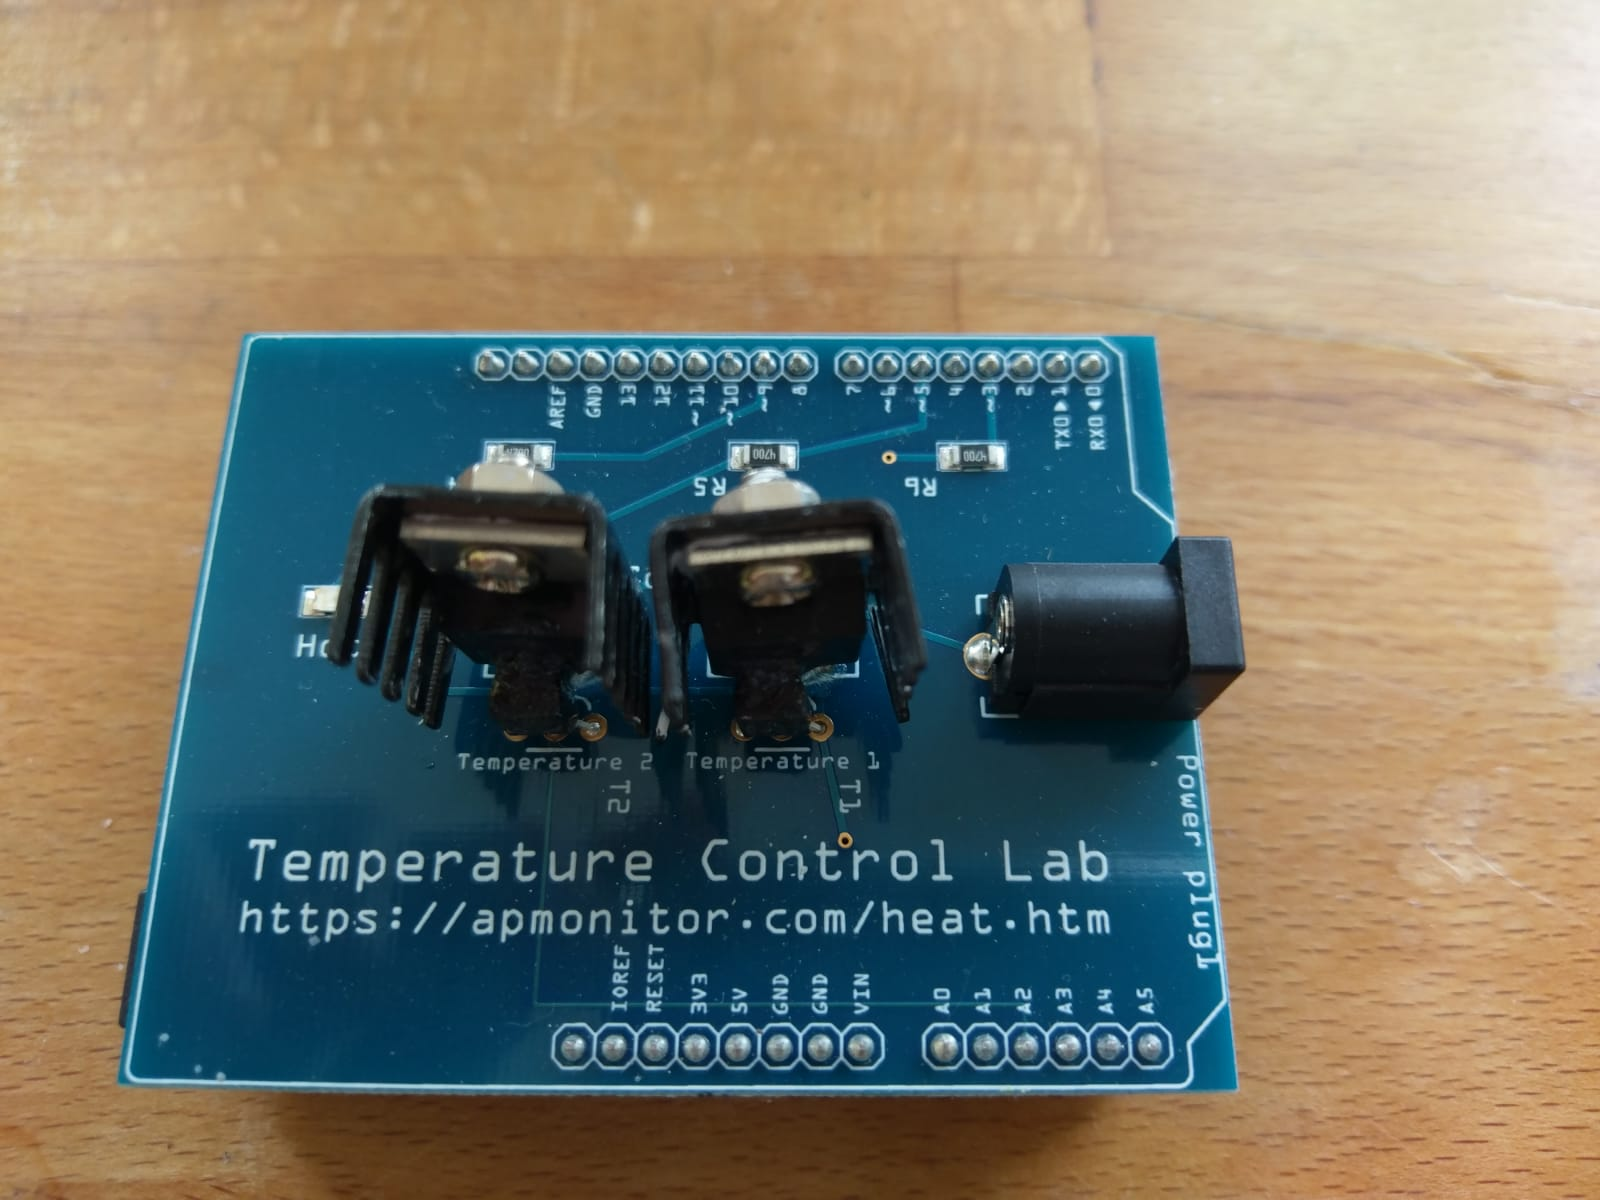
\includegraphics[width = 0.8\textwidth]{Latex/images/Introduction/Setup.jpeg}
    \caption{The setup of the heater system}
    \label{fig:setup}
\end{figure}
First, the system will be investigated. This will consist of a linearity test and two different methods for system identification. These models will be used to design state observers. Finally, two different control approaches will be used to control the temperature of the heaters. The different methods and approaches will be compared and discussed.